
\documentclass[xcolor={dvipsnames}]{beamer}
\usepackage{amsmath,amsfonts,amssymb,pxfonts,eulervm,xspace}
\usepackage{graphicx}
 \usepackage{multimedia}
\usepackage{media9}
\usepackage{minted}

\usepackage{animate}

\graphicspath{{./figures/}}
\usetheme{ccnycrest}


\newenvironment{changemargin}[2]{%
\begin{list}{}{%
\setlength{\topsep}{0pt}%
\setlength{\leftmargin}{#1}%
\setlength{\rightmargin}{#2}%
\setlength{\listparindent}{\parindent}%
\setlength{\itemindent}{\parindent}%
\setlength{\parsep}{\parskip}%
}%
\item[]}{\end{list}}

\begin{document}

\title{ CS102: While and Do While Loops }
\author{Hannah Aizenman}
\date{haizenm00@ccny.cuny.edu}


\begin{frame}
	\titlepage
\end{frame}

\begin{frame}{Making a Pretzel}
	\begin{center}
		\animategraphics[height=3in,autoplay,controls]{12}{assembly/animate_}{000}{271}
	\end{center}
\end{frame}

\begin{frame}{1 Pretzel}
	\begin{figure}
		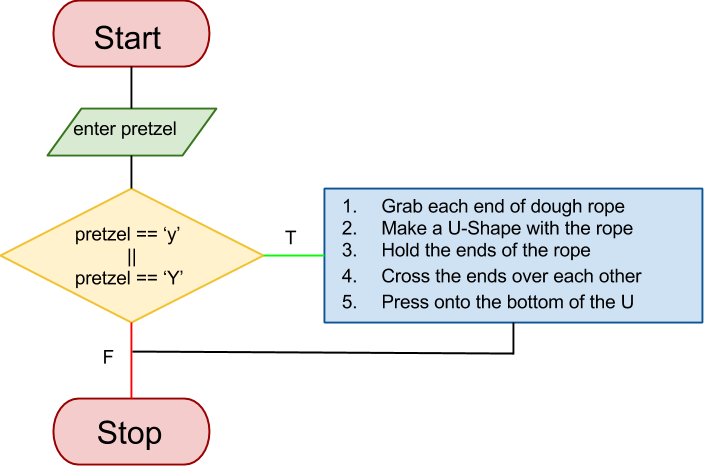
\includegraphics[width=.8\textwidth]{if_pretzel}
	\end{figure}
\end{frame}

%
\begin{frame}[fragile]{Make A Pretzel?}
\begin{minted}{c++}
#include<iostream>
using namespace std;

int main(){
    char pretzel;
    cout<<"Would you like a pretzel?"<<endl;
    cin>>pretzel;
    if(pretzel == 'y' || pretzel =='Y'){
       cout<<"Grab each end of dough rope"<<endl;
       cout<<"Make a U-Shape with the rope"<<endl;
       cout<<"Hold the ends of the rope"<<endl;
       cout<<"Cross the ends over each other"<<endl;
       cout<<"Press onto the bottom of the U"<<endl;
    }
    return 0;
}
\end{minted}
\end{frame}


\begin{frame}{Make Lots of Pretzels}
	\begin{figure}
		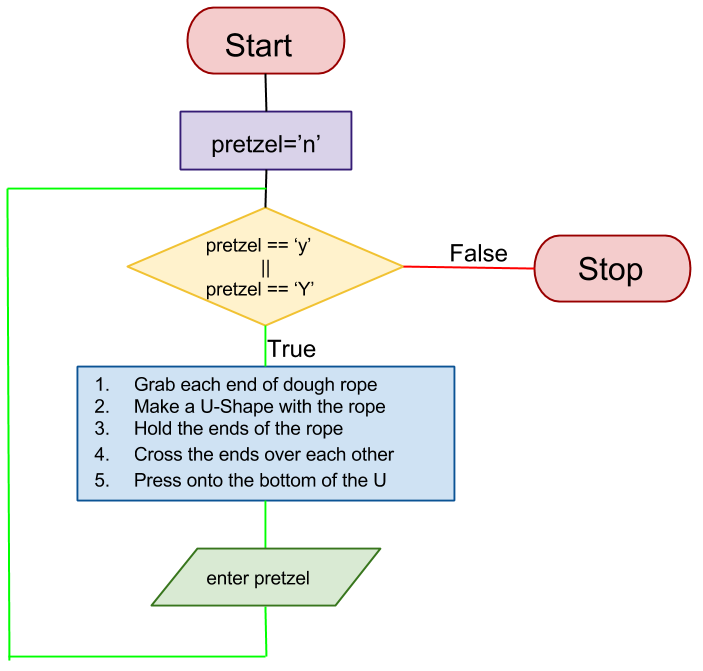
\includegraphics[width=.75\textwidth]{while_pretzels}
	\end{figure}
\end{frame}

%
\begin{frame}[fragile]{Make Lots of  Pretzels?}
\begin{minted}{c++}
    char pretzel = 'y';

    cout<<"Would you like a pretzel?"<<endl;
    cin>>pretzel;

    while(pretzel == 'y' || pretzel =='Y'){
       cout<<"Grab each end of dough rope"<<endl;
       cout<<"Make a U-Shape with the rope"<<endl;
       cout<<"Hold the ends of the rope"<<endl;
       cout<<"Cross the ends over each other"<<endl;
       cout<<"Press onto the bottom of the U"<<endl;       

       cout<<"Would you like a pretzel?"<<endl;
       cin>>pretzel;
    }
\end{minted}
\end{frame}

\begin{frame}{Practice While Loops}
\begin{enumerate}
	\item Write a program that reads numbers until number is less than or equal to 100.
	\item Find the minimum of the numbers being read in. 
	\item Find the maxmium.
	\item Find the average.
\end{enumerate}
\end{frame}

\begin{frame}{Make At Least 1 Pretzel}
	\begin{figure}
		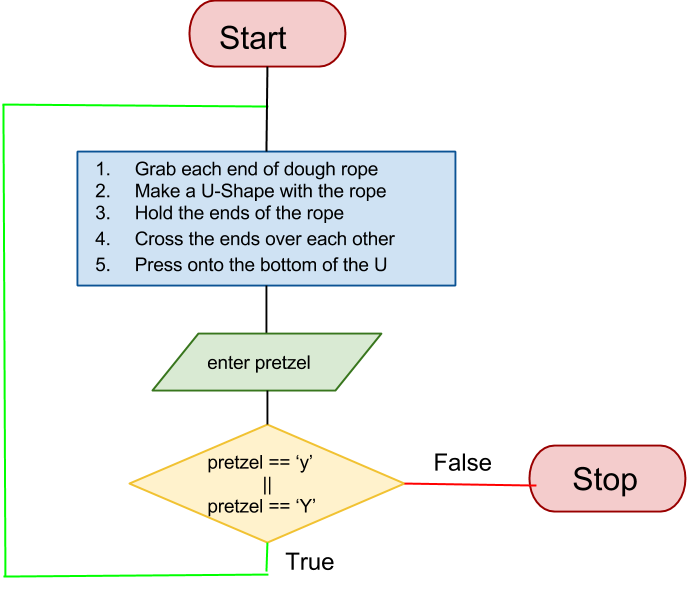
\includegraphics[width=.8\textwidth]{do_while_pretzels}
	\end{figure}
\end{frame}

%
\begin{frame}[fragile]{Make Lots of  Pretzels?}
\begin{minted}{c++}
    char pretzel;

    do{     
       cout<<"Grab each end of dough rope"<<endl;
       cout<<"Make a U-Shape with the rope"<<endl;
       cout<<"Hold the ends of the rope"<<endl;
       cout<<"Cross the ends over each other"<<endl;
       cout<<"Press onto the bottom of the U"<<endl;

       cout<<"Would you like a pretzel?"<<endl;
       cin>>pretzel;
    }while(pretzel == 'y' || pretzel =='Y');
 
\end{minted}
\end{frame}

\begin{frame}{Practice Do While Loops}
\begin{itemize}
	\item Machine epsilon is the smallest positive floating point number such that 1.0 + machine epsilon is not equal to 1.0. Epsilon can be approximated by repeatedly dividing a number by 2. Write a program to calculate epsilon. 
	\item
\end{itemize}
\end{frame}

\begin{frame}{Break out of Loop}
	\begin{figure}
		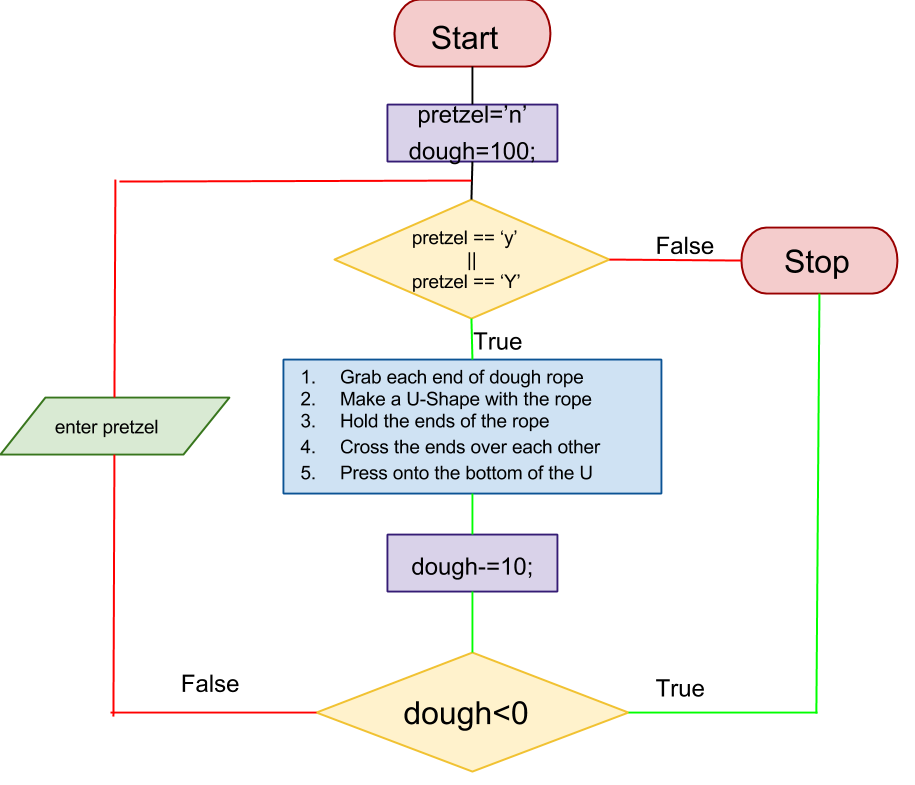
\includegraphics[width=.8\textwidth]{break_pretzels}
	\end{figure}
\end{frame}

\begin{frame}[fragile]{Break Statement}
\begin{minted}{c++}
    char pretzel = 'y';
    int dough == 100;
    cout<<"Would you like a pretzel?"<<endl;
    cin>>pretzel;

    while(pretzel == 'y' || pretzel =='Y'){
       cout<<"Grab each end of dough rope"<<endl;
       cout<<"Make a U-Shape with the rope"<<endl;
       cout<<"Hold the ends of the rope"<<endl;
       cout<<"Cross the ends over each other"<<endl;
       cout<<"Press onto the bottom of the U"<<endl; 
       dough-=10;
       if(dough<0){
          break;     
       }
       cout<<"Would you like a pretzel?"<<endl;
       cin>>pretzel;
    }
\end{minted}
\end{frame}

\begin{frame}{Make At Least 1 Pretzel}
	\begin{figure}
		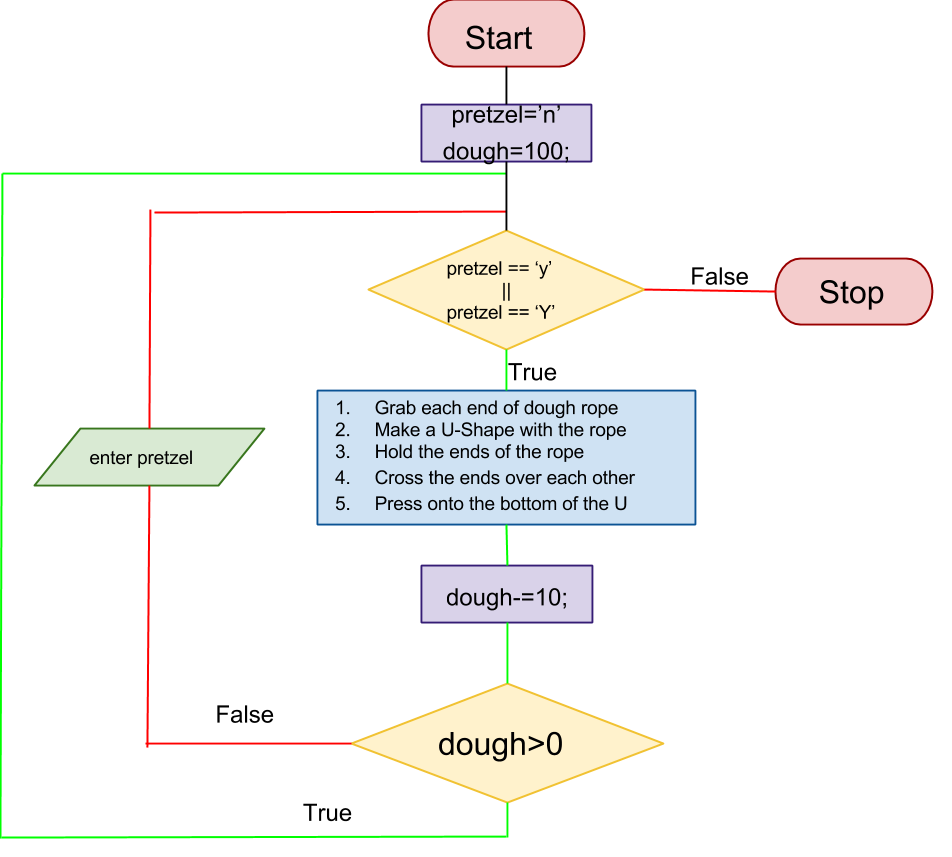
\includegraphics[width=.8\textwidth]{continue_pretzels}
	\end{figure}
\end{frame}


\begin{frame}[fragile]{Continue Statement}
\begin{minted}{c++}
    char pretzel = 'y';
    int dough = 100;
    cout<<"Would you like a pretzel?"<<endl;
    cin>>pretzel;

    while(pretzel == 'y' || pretzel =='Y'){
       cout<<"Grab each end of dough rope"<<endl;
       cout<<"Make a U-Shape with the rope"<<endl;
       cout<<"Hold the ends of the rope"<<endl;
       cout<<"Cross the ends over each other"<<endl;
       cout<<"Press onto the bottom of the U"<<endl; 
       dough-=10;
       if(dough>0){
          continue;     
       }
       cout<<"Would you like a pretzel?"<<endl;
       cin>>pretzel;
    }
\end{minted}
\end{frame}

\begin{frame}[fragile]{Infinite Loops}
	\begin{description}
	\item[no range]
	\begin{minted}{c++}
		for(;;){cout<<"hello";}
	\end{minted}

	\item[always true]
	\begin{minted}{c++}
		while(true){cout<<"world";};
	\end{minted}
	\item[always true]
	\begin{minted}{c++}
		do{cout<<"!"<<endl;}while(1);
	\end{minted}

	\item[k \& i increase]
	\begin{minted}{c++}
	     k=10;
	     for(int i=0; i<k; i++){k+=i};
	\end{minted}

	\item[always i \textgreater 0]
	\begin{minted}{c++}
	     int =10;
	     while(i>=0){i/=2};
	\end{minted}
	
	\item[no change]
	\begin{minted}{c++}
	     stop = 'N'
	     do{ cout<<"quit";}{while{stop!='Y'};
	\end{minted}

	\end{description}
	
\end{frame}

\end{document}

